\documentclass[a4paper,12pt]{report}
\usepackage[T2A]{fontenc}
\usepackage[utf8]{inputenc}
\usepackage[english,russian]{babel}
\usepackage{geometry}
\usepackage{listings}
\geometry{top=2cm}
\usepackage{titlesec}
\usepackage{blindtext}
\usepackage{color}
\usepackage{pgfplots}
\usepackage{filecontents}
\usetikzlibrary{datavisualization}
\usetikzlibrary{datavisualization.formats.functions}
\usepackage{caption}
\DeclareCaptionFont{white}{\color{white}}
\captionsetup[table]{position=bottom}
\DeclareCaptionFormat{listing}{\colorbox{gray}{\parbox{\textwidth}{#1#2#3}}}
\captionsetup[lstlisting]{format=listing,labelfont=white,textfont=white}

% Для листинга кода:
\lstset{ %
language=Python,                 % выбор языка для подсветки
basicstyle=\small\sffamily, % размер и начертание шрифта для подсветки кода
numbers=left,               % где поставить нумерацию строк (слева\справа)
numberstyle=\tiny,           % размер шрифта для номеров строк
stepnumber=1,                   % размер шага между двумя номерами строк
numbersep=-5pt,                % как далеко отстоят номера строк от подсвечиваемого кода
showspaces=false,
backgroundcolor=\color{white},         
showstringspaces=false,      % показывать или нет пробелы в строках
showtabs=false,             % показывать или нет табуляцию в строках
frame=single,              % рисовать рамку вокруг кода
tabsize=2,                 % размер табуляции по умолчанию равен 2 пробелам
captionpos=t,              % позиция заголовка вверху [t] или внизу [b] 
breaklines=true,           % автоматически переносить строки (да\нет)
breakatwhitespace=false, % переносить строки только если есть пробел
escapeinside={\%*}{*)},   % если нужно добавить комментарии в коде
	    keywordstyle=\color{blue}\ttfamily,
	    stringstyle=\color{red}\ttfamily,
	    commentstyle=\color{green}\ttfamily,
	    morecomment=[l][\color{magenta}]{\#},
	    columns=fullflexible   % если нужно добавить комментарии в коде
}

% Для измененных титулов глав:
\definecolor{gray75}{gray}{0.75} % определяем цвет
\newcommand{\hsp}{\hspace{20pt}} % длина линии в 20pt
% titleformat определяет стиль
\titleformat{\chapter}[hang]{\Huge\bfseries}{\thechapter\hsp\textcolor{gray75}{|}\hsp}{0pt}{\Huge\bfseries}


% Графики
\begin{filecontents}{LevMatr.dat}
100 0.0045225
200 0.0223677
300 0.0646862
400 0.1469188
500 0.2822859
600 0.4822320
700 0.7579869
800 1.1269531
900 1.5967085
1000 2.1819938
\end{filecontents}

\begin{filecontents}{DamMatr1.dat}
100 0.0055206
200 0.0273994
300 0.0793424
400 0.1807984
500 0.3479397
600 0.5953705
700 0.9377318
800 1.3960131
900 1.9797975
1000 2.7077450
\end{filecontents}

\begin{filecontents}{DamRec.dat}
1 0.0000019
2 0.0000094
3 0.0000442
4 0.0002221
5 0.0011502
6 0.0061078
7 0.0329801
8 0.1799263
9 0.9907548
10 5.4900566
\end{filecontents}

\begin{filecontents}{DamMatr2.dat}
1 0.0000023
2 0.0000067
3 0.0000139
4 0.0000256
5 0.0000430
6 0.0000681
7 0.0001034
8 0.0001521
9 0.0002132
10 0.0002846
\end{filecontents}


\begin{document}
\begin{titlepage}
	\centering
	{\scshape\LARGE МГТУ им. Баумана \par}
	\vspace{4cm}
	{\scshape\Large Лабораторная работа №1\par}
	\vspace{0.5cm}	
	{\scshape\Large По курсу: "Анализ алгоритмов"\par}
	\vspace{2cm}
	{\huge\bfseries Расстояние Левенштейна\par}
	\vspace{3cm}
	\Large Работу выполнил: Лумбунов Дмитрий, ИУ7-54Б\par
	\vspace{0.5cm}
	\Large Преподаватель:  Волкова Л.Л., Строганов Ю.В.\par

	\vfill
	\large \textit {Москва, 2019} \par
\end{titlepage}

\setcounter{page}{2}

\tableofcontents

\newpage
\chapter*{Введение}
\addcontentsline{toc}{chapter}{Введение}
\hspace{0.6cm} \textbf{Расстояние Левенштейна} (также редакционное расстояние или дистанция редактирования) — это минимальное количество операций вставки одного символа, удаления одного символа и замены одного символа на другой, необходимых для превращения одной строки в другую.

Впервые задачу поставил в 1965 году советский математик Владимир Иосифович Левенштейн при изучении последовательностей 0-1. Впоследствии более общую задачу для произвольного алфавита связали с его именем. Большой вклад в изучение вопроса внёс Дэн Гасфилд.

Расстояние Левенштейна и его обобщения активно применяется для исправления ошибок в слове (в поисковых системах, базах данных, при вводе текста, при автоматическом распознавании отсканированного текста или речи); для сравнения текстовых файлов утилитой diff и ей подобными; в биоинформатике для сравнения генов, хромосом и белков.

\textbf{Расстояние Дамерау — Левенштейна} (названо в честь учёных Фредерика Дамерау и Владимира Левенштейна) — это мера разницы двух строк символов, определяемая как минимальное количество операций вставки, удаления, замены и транспозиции (перестановки двух соседних символов), необходимых для перевода одной строки в другую. Является модификацией расстояния Левенштейна: к операциям вставки, удаления и замены символов, определённых в расстоянии Левенштейна добавлена операция транспозиции (перестановки) символов. Расстояние Дамерау-Левенштейна, как и метрика Левенштейна, является мерой "схожести" двух строк. Алгоритм его поиска находит применение в реализации нечёткого поиска, а также в биоинформатике (сравнение ДНК), несмотря на то, что изначально алгоритм разрабатывался для сравнения текстов, набранных человеком (Дамерау показал, что 80\% человеческих ошибок при наборе текстов составляют перестановки соседних символов, пропуск символа, добавление нового символа, и ошибка в символе. Поэтому метрика Дамерау-Левенштейна часто используется в редакторских программах для проверки правописания).

\newpage
\textbf{\LARGE Задачи работы}\\\\
Задачами данной лабораторной являются:
\begin{enumerate}
  	\item изучение алгоритмов Левенштейна и Дамерау-Левенштейна нахождения расстояния между строками;
	\item получение практических навыков реализации указанных алгоритмов: двух алгоритмов в матричной версии и одного из алгоритмов в рекурсивной версии; 
	\item сравнительный анализ линейной и рекурсивной реализаций выбранного алгоритма определения расстояния между строками по затрачиваемым ресурсам (времени и памяти); 
	\item экспериментальное подтверждение различий во временнóй эффективности рекурсивной и
нерекурсивной реализаций выбранного алгоритма определения расстояния между строками при
помощи разработанного программного обеспечения на материале замеров процессорного времени
выполнения реализации на варьирующихся длинах строк; 
	\item описание и обоснование полученных результатов в отчете о выполненной лабораторной
работе, выполненного как расчётно-пояснительная записка к работе. 
\end{enumerate}


\chapter{Аналитическая часть}
В этом разделе содержатся описания алгоритмов нахождения расстояний Левенштейна и Дамерау-Левенштейна и их практическое применение.
\section{Расстояние Левенштейна}
\hspace{0.6cm}\textbf {Расстояние Левенштейна} - это минимальное количество операций вставки одного символа, удаления одного символа и замены одного символа на другой, необходимых для превращения одной строки в другую.\\
    
Каждая операция имеет свой вес (штраф). Редакционным предписанием называется последовательность действий, необходимых для получения из первой строки вторую, и минимизирующую суммарную цену. Суммарная цена есть искомое расстояние Левенштейна.\\
 
\textbf{Введем следующие обозначения операций:} 
\begin{enumerate}
  	\item D (delete) — удалить,
	\item I (insert) — вставить,
	\item R (replace) — заменить,
	\item M (match) - совпадение.
\end{enumerate}

Пусть $S_{1}$ и $S_{2}$ — две строки (длиной M и N соответственно) над некоторым алфавитом, тогда расстояние Левенштейна можно подсчитать по следующей рекуррентной формуле:

\begin{displaymath}
D(i,j) = \left\{ \begin{array}{ll}
 0,  \textrm{$i = 0, j = 0$}\\
 i,  \textrm{$j = 0, i > 0$}\\
 j,  \textrm{$i = 0, j > 0$}\\
min\left\{ \begin{array}{ll}
D(s1[1..i],s2[1..j-1]) + 1,\\
D(s1[1..i-1],s2[1..j]) + 1,\\
D(s1[1..i-1],s2[1..j-1]) + (S1[i] == S2[j] ? 0 : 1))\\
\end{array} \right.
  \end{array} \right.
\end{displaymath}

, где 1 - вставка символа, 2 - удаление символа, 3 - замена символа, при этом, если $S1[i - 1] = S2[j - 1]$, то вес такой операции будет равен 0, иначе 1.

Существует 2 основных способа нахождения расстояния Левенштейна:\\матричный и рекурсивный.


Для нахождения кратчайшего расстояния матричным способом необходимо вычислить матрицу D, используя вышеприведённую формулу. Матрица размером $(length(S1)+ 1)$x$((length(S2) + 1)$, где $length(S)$ — длина строки S. Значение в ячейке $[i, j]$ равно значению $D(S1[1...i], S2[1...j])$. Первая строка и первый столбец тривиальны. В соответствии с формулой получаем: $A[i][j] = min (A[i-1][j] + 1, A[i][j-1] + 1, A[i-1][j-1] + m(S1[i], S2[j]))$, где $m(S1[i], S2[j])$ — функция, равная 0 при $S1[i - 1] = S2[j - 1]$ и 1 в обратном случае. В результате расстоянием Левенштейна будет ячейка матрицы с индексами $i = length(S1$) и $j = length(S2)$.
Для восстановления редакционного предписания требуется вычислить матрицу D, после чего идти из правого нижнего угла в левый верхний, на каждом шаге находя минимальное из трёх значений:
    \begin{itemize}
    \item если минимально $(D(i-1, j)$ + цена удаления символа $S1[i]$), добавляем удаление символа $S1[i]$ и идём в $[i-1, j]$;
    \item если минимально $(D(i, j-1)$ + цена вставки символа $S2[j]$), добавляем вставку     символа $S2[j]$ и идём в $[i, j-1]$;
    \item если минимально $(D(i-1, j-1)$ + цена замены символа $S1[i]$ на символ $S2[j]$),     добавляем замену $S1[i]$ на $S2[j]$ (если они не равны; иначе ничего не добавляем), после чего идём в $[i-1, j-1]$.
	\end{itemize}

Второй способ нахождения расстояния Левенштейна - рекурсивно в соответствии с формулами, обрабатывая подстроки, пока не будет достигнут тривиальный случай. Работать с подстроками затратно по объему памяти, также в рекурсивном алгоритме будут обрабатываться одинаковые случаи несколько раз, что неэффективно по памяти и по времени.

\section{Расстояние Дамерау-Левенштейна}
\hspace{0.6cm}\textbf{Расстояние Дамерау-Левенштейна} - это мера разницы двух строк символов, определяемая как минимальное количество операций вставки, удаления, замены и транспозиции (перестановки двух соседних символов), необходимых для перевода одной строки в другую. Является модификацией расстояния Левенштейна: к операциям вставки, удаления и замены символов, определённых в расстоянии Левенштейна добавлена операция транспозиции (перестановки) символов.

Расстояние Дамерау-Левенштейна вычисляется по следующей рекуррентной формуле:

\begin{displaymath}
D(i,j) = \left\{ \begin{array}{ll}
 0,  \textrm{$i = 0, j = 0$}\\
 i,  \textrm{$j = 0, i > 0$}\\
 j,  \textrm{$i = 0, j > 0$}\\
min\left\{ \begin{array}{ll}
D(s1[1..i],s2[1..j-1]) + 1,\\
D(s1[1..i-1],s2[1..j]) + 1,\\
D(s1[1..i-1],s2[1..j-1]) + (S1[i] == S2[j] ? 0 : 1)),\\
D(s1[1..i-2],s2[1..j-2]) + 1, \\ \hspace{1cm}\textrm{if $i,j>1$ and $s1[i] = s2[j-1],s1[i-1]=s2[j] $}\\
\end{array} \right.
  \end{array} \right.
\end{displaymath}
, где 1 - вставка символа, 2 - удаление символа, 3 - замена символа, при этом, если $S1[i - 1] = S2[j - 1]$, то вес такой операции будет равен 0, иначе 1,\\ 4 - перестановка символов в  случае, если $S1[i-1] = S2[j]$ и $S1[i] = S2[j-1]$.

Решения задачи нахождения расстояния Дамерау-Левенштейна аналогичны решениям задачи нахождения расстояния Левенштейна. 

При матричной реализации формула для ячейки [i,j] модифицируется следующим образом: $A[i][j] = min (A[i-1][j] + 1, A[i][j-1] + 1, A[i-1][j-1] + m(s1[i], s2[j]), A[i - 2][j - 2] + 1$, если $s1[i] = s2[j-1]$ и $ s1[i-1] = s2[j]$ и $i > 1$ и $j > 1$. Для восстановления редакционного предписания требуется вычислить матрицу $D$, после чего идти из правого нижнего угла в левый верхний, на каждом шаге ища минимальное из четырех значений:
\begin{itemize}
    \item если минимально $(D(i-1, j)$ + цена удаления символа $S1[i]$), добавляем удаление символа $S1[i]$ и идём в $[i-1, j]$;
    \item если минимально $(D(i, j-1)$ + цена вставки символа $S2[j]$), добавляем вставку     символа $S2[j]$ и идём в $[i, j-1]$;
    \item если минимально $(D(i-1, j-1)$ + цена замены символа $S1[i]$ на символ $S2[j]$),     добавляем замену $S1[i]$ на $S2[j]$ (если они не равны; иначе ничего не добавляем), после чего идём в $[i-1, j-1]$
    \item если транспозиция возможна, то возвращаем $(D(i-2, j-2) + 1$
\end{itemize}

При рекурсивном решении добавляется еще одна ветвь в дерево рекурсий,когда проверяется условие того, что два заключительных символа очередной подстроки равны двум другим из второй подстроки с учетом транспозиции.

\section{Практическое применение}
Данные алгоритмы применяются при поиске информации по запросу, с помощью них можно найти наиболее подходящее(имеющее наименьшее расстояние) к нему слово и заменить его в поисковой строке. Метод оценки редакционного расстояния активно применяется в биоинформатике для сравнения генов, хромосом и белков.

\chapter{Конструкторская часть}
В этом разделе содержатся cхемы алгоритмов нахождения расстояний Левенштейна и Дамерау-Левенштейна и сравнительный анализ матричной и рекурсивной реализаций.
\newpage
\section{Схемы алгоритмов}

\hspace{0.6cm}На Рис.2.1 и 2.2 представлена схема матричного алгоритма нахождения расстояния Левенштейна.
\begin{figure}[ht!]
\center{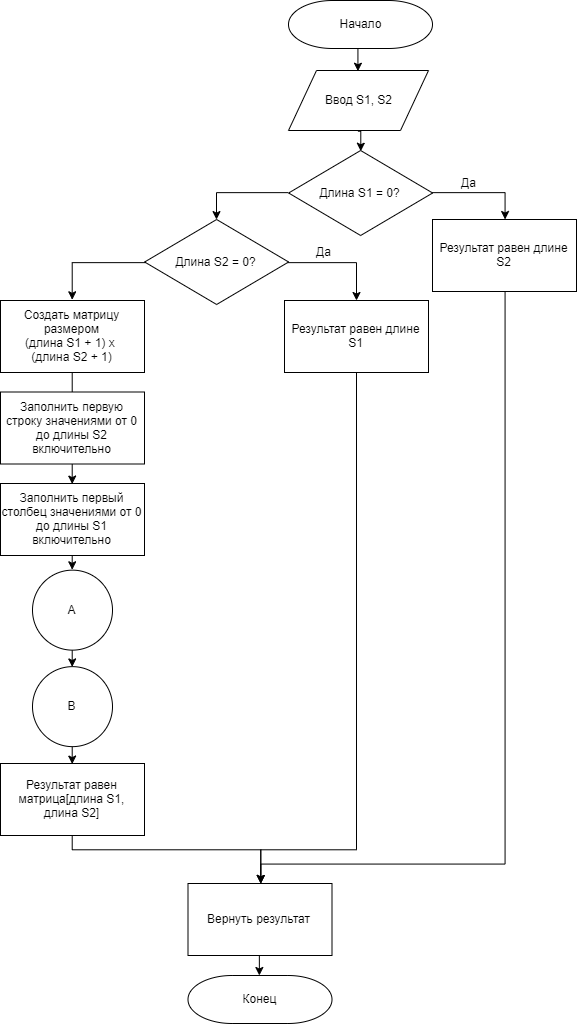
\includegraphics[scale=0.56]{LevMatr1.png}}
\caption{Матричный алгоритм нахождения расстояния Левенштейна}
\end{figure}
\newpage
\begin{figure}[ht!]
\center{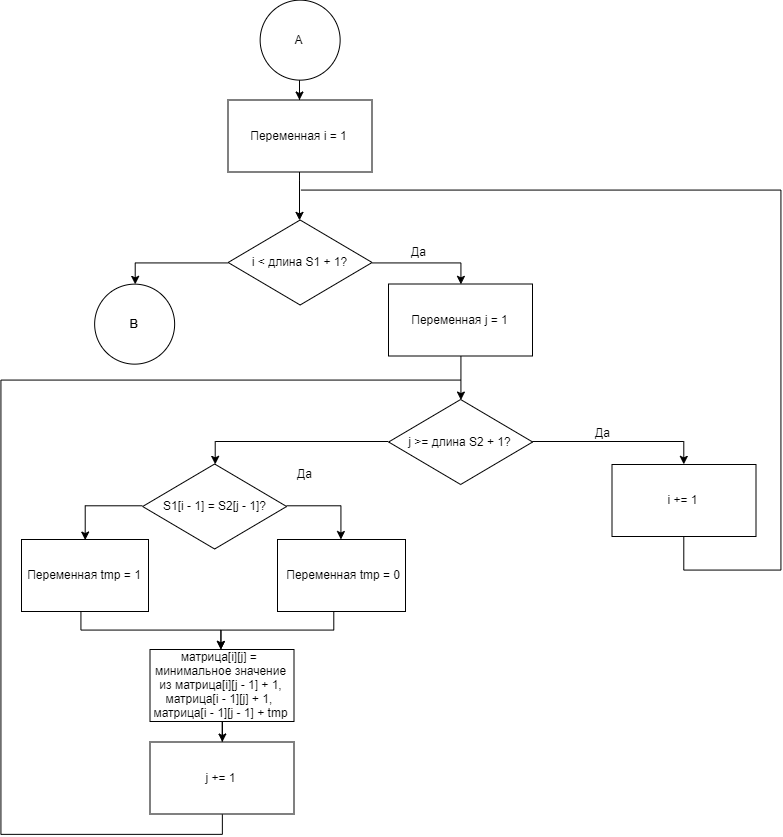
\includegraphics[scale=0.6]{LevMatr2.png}}
\caption{Матричный алгоритм нахождения расстояния Левенштейна (продолжение)}
\end{figure}
\newpage
На Рис.2.3 и 2.4 представлена схема матричного алгоритма нахождения расстояния Дамерау-Левенштейна.
\begin{figure}[ht!]
\center{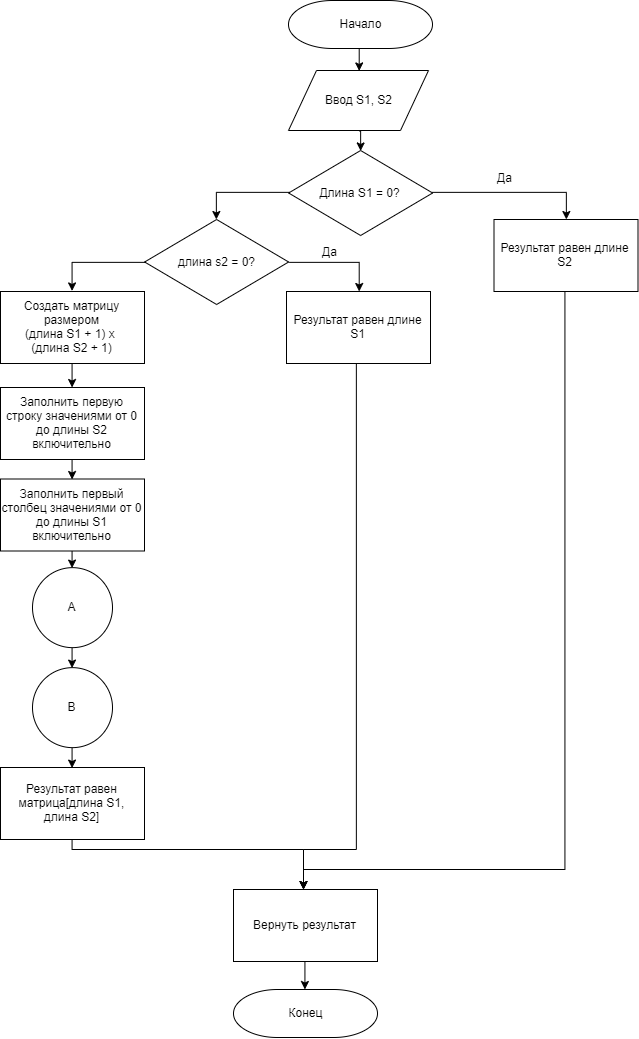
\includegraphics[scale=0.56]{DamMatr1.png}}
\caption{Матричный алгоритм нахождения расстояния Дамерау-Левенштейна}
\end{figure}
\begin{figure}[ht!]
\center{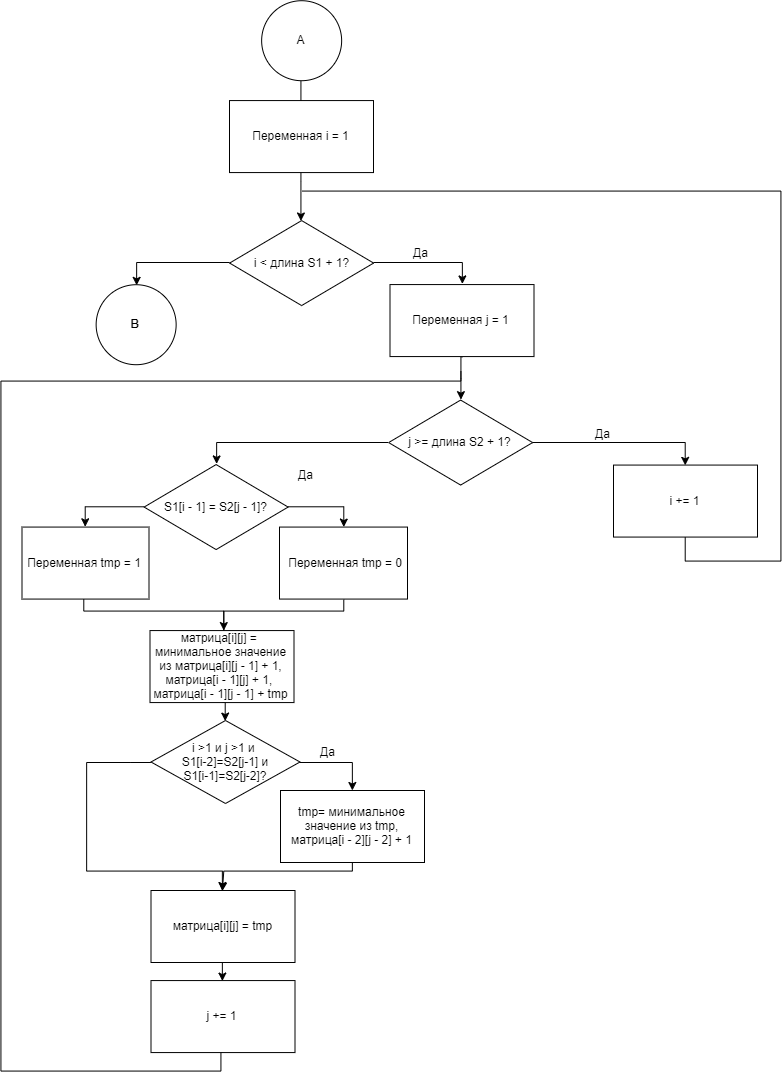
\includegraphics[scale=0.57]{DamMatr2.png}}
\caption{Матричный алгоритм нахождения расстояния Дамерау-Левенштейна (продолжение)}
\end{figure}
\newpage
\newpage
На Рис.2.5 представлена схема рекурсивного алгоритма нахождения расстояния Дамерау-Левенштейна.
\begin{figure}[ht!]
\center{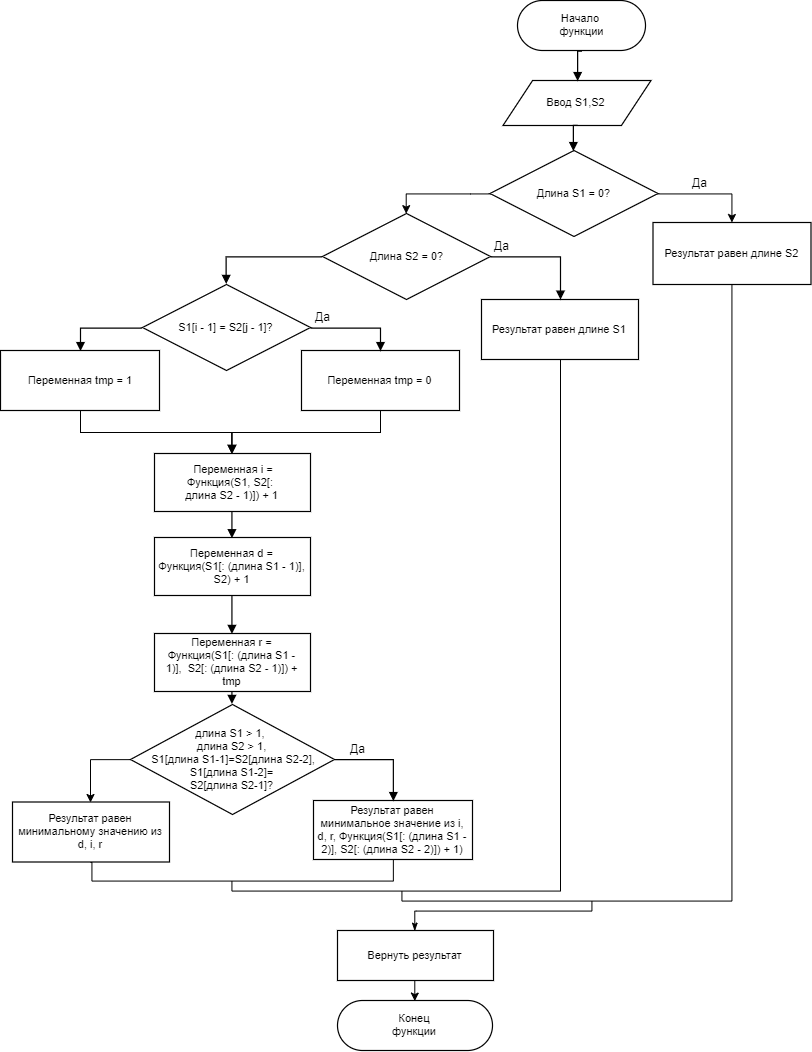
\includegraphics[scale=0.57]{DamRec.png}}
\caption{Рекурсивный алгоритм нахождения расстояния Дамерау-Левенштейна}
\end{figure}
\newpage
\section{Сравнительный анализ матричной и рекурсивной реализаций}
Рекурсивная реализация работает медленнее по сравнению с матричной из-за повторных вычислений, возникающих в ходе работы рекурсивного алгоритма. Это наглядно видно на Рис.2.6, иллюстрирующем дерево рекурсивных вызовов. При каждом рекурсивном вызове необходимо передавать в функцию подстроки исходных строк, что затратно по памяти. Эту проблему возможно избежать, если занести строки в глобальные переменные, что является плохой практикой. 

\begin{figure}[ht!]
\center{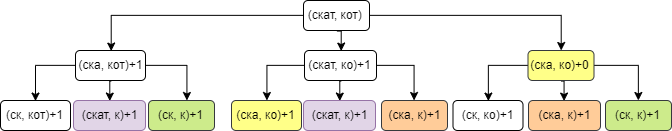
\includegraphics[scale=0.7]{rec.png}}
\caption{Дерево рекурсивных вызовов}
\end{figure}

Для сравнения, вызов функции, которая реализует матричный алгоритм, происходит один раз и в функцию только один раз передаются обе строки. В этом алгоритме память будет затрачена на хранение матрицы, а время на вложенные циклы, однако затраты будут существенно меньше, чем при многократных вызовах рекурсивной функции.
	
Пусть длина строки S1 - n, длина строки S2 - m, тогда затраты памяти на приведенные выше алгоритмы будут следующими:
\begin{itemize}
\item матричный алгоритм Левенштейна:\begin{itemize}
	\item строки S1, S2 - (m + n) * sizeof(char)
	\item матрица - ((m + 1) * (n + 1)) * sizeof(int)
	\item текущая строка матрицы - (n + 1) * sizeof(int)
	\item длины строк - 2 * sizeof(int)
	\item вспомогательные переменные -  3 * sizeof(int)
	\end{itemize}
\item матричный алгоритм Дамерау-Левенштейна:\begin{itemize}
	\item строки S1, S2 - (m + n) * sizeof(char)
	\item матрица - ((m + 1) * (n + 1)) * sizeof(int)
	\item текущая строка матрицы - (n + 1) * sizeof(int)
	\item длины строк - 2 * sizeof(int)
	\item вспомогательные переменные -  3 * sizeof(int)
	\end{itemize}
\newpage
\item рекурсивный алгоритм Дамерау-Левенштейна(для каждого вызова):\begin{itemize}
	\item строки S1, S2 - (m + n) * sizeof(char)
	\item длины строк - 2 * sizeof(int)
	\item вспомогательная переменная -  sizeof(int)
	\item адрес возврата
	\end{itemize}
\end{itemize}

\chapter{Технологическая часть}
В данном разделе приведены требования к программнму обеспечению, средства реализации и листинг кода
\section{Требования к ПО}
Программа на вход получает две строки символов. Результат работы программы: число - искомое расстояние. Для матричных реализаций дополнительно выводится получившаяся в результате работы программы матрица.

\section{Средства реализации}
Для реализации представленных алгоритмов был выбран язык Python. Время работы алгоритмов было замерено с помощью функции time() из библиотеки time.

\section{Листинги кода}

\hspace{0.6cm}В Листинге 3.1 показана реализация матричного алгоритма нахождения расстояния Левенштейна
\begin{lstlisting}[caption=Функция нахождения расстояния Левенштейна матрично]
def levenshtein_matrix(s1, s2, matrix_flag):
    n, m = len(s1), len(s2)
    current_row = range(n + 1)
    matrix = [current_row]
    for i in range(1, m + 1):
        current_row = [i] + [0] * n
        for j in range(1, n + 1):
            current_row[j] = matrix[i - 1][j - 1]
            if s1[j - 1] != s2[i - 1]:
                current_row[j] += 1
            current_row[j] = min(current_row[j], matrix[i-1][j] + 1,
                                 current_row[j - 1] + 1)
        matrix.append(current_row)
    if matrix_flag:
        print_matrix(matrix)
    return matrix[m][n]
\end{lstlisting}

В Листинге 3.2 показана реализация матричного алгоритма нахождения расстояния Дамерау-Левенштейна
\begin{lstlisting}[caption=Функция нахождения расстояния Дамерау-Левенштейна матрично]
def damerau_levenshtein_matrix(s1, s2, matrix_flag):
    n, m = len(s1), len(s2)
    current_row = range(n + 1)
    matrix = [current_row]
    for i in range(1, m + 1):
        current_row = [i] + [0] * n
        for j in range(1, n + 1):
            current_row[j] = matrix[i - 1][j - 1]
            if s1[j - 1] != s2[i - 1]:
                current_row[j] += 1
            current_row[j] = min(current_row[j], matrix[i-1][j] + 1,
                                 current_row[j - 1] + 1)
            if i > 1 and j > 1 and s1[j - 1] == s2[i - 2] \
                    and s1[j - 2] == s2[i - 1]:
                current_row[j] = min(current_row[j],
                                     matrix[i - 2][j - 2] + 1)
        matrix.append(current_row)
    if matrix_flag:
        print_matrix(matrix)
    return matrix[m][n]
\end{lstlisting}

В Листинге 3.3 показана реализация рекурсивного алгоритма нахождения расстояния Дамерау-Левенштейна
\begin{lstlisting}[caption=Функция нахождения расстояния Дамерау-Левенштейна рекурсивно]
def damerau_levenshtein_recursive(s1, s2):
    n, m = len(s1), len(s2)
    if n == 0 or m == 0:
        if n != 0:
            return n
        if m != 0:
            return m
        return 0
    change = 0
    if s1[-1] != s2[-1]:
        change += 1
    if n > 1 and m > 1 and s1[-1] == s2[-2] and s1[-2] == s2[-1]:
        return min(damerau_levenshtein_recursive(s1[:n - 1], s2)
                   + 1,
                   damerau_levenshtein_recursive(s1, s2[:m - 1])
                   + 1,
                   damerau_levenshtein_recursive(s1[:n - 1],
                                                 s2[:m - 1])
                   + change,
                   damerau_levenshtein_recursive(s1[:n - 2],
                                                 s2[:m - 2]) + 1)
    else:
        return min(damerau_levenshtein_recursive(s1[:n - 1], s2)
                   + 1,
                   damerau_levenshtein_recursive(s1, s2[:m - 1])
                   + 1,
                   damerau_levenshtein_recursive(s1[:n - 1],
                                                 s2[:m - 1])
                   + change)
\end{lstlisting}



\chapter{Эксперементальная часть}
В данном разделе приведены примеры работы программы, постановка эксперимента и сравнительный анализ алгоритмов на основе экспериментальных данных.
\section{Примеры работы}
\textbf {Пример 1}\\
Строка s1 = кот\\
Строка s2 = скат\\
Расстояние Левенштейна(матричный алгоритм): 2\\
0 1 2 3\\
1 1 2 3\\
2 1 2 3\\
3 2 2 3\\
4 3 3 2\\
Расстояние Дамерау-Левенштейна(матричный алгоритм):2\\
0 1 2 3\\
1 1 2 3\\
2 1 2 3\\
3 2 2 3\\
4 3 3 2\\
Расстояние Дамерау-Левенштейна(рекурсивный алгоритм):2\\\\
\textbf {Пример 2}\\
Строка s1 = отчет\\
Строка s2 = спать\\
Расстояние Левенштейна(матричный алгоритм): 5\\
0 1 2 3 4 5\\
1 1 2 3 4 5\\
2 2 2 3 4 5\\
3 3 3 3 4 5\\
4 4 3 4 4 4\\
5 5 4 4 5 5\\
Расстояние Дамерау-Левенштейна(матричный алгоритм):5\\
0 1 2 3 4 5\\
1 1 2 3 4 5\\
2 2 2 3 4 5\\
3 3 3 3 4 5\\
4 4 3 4 4 4\\
5 5 4 4 5 5\\
Расстояние Дамерау-Левенштейна(рекурсивный алгоритм):5\\\\
\textbf {Пример 3}\\
Строка s1 = кофе\\
Строка s2 = коеф\\
Расстояние Левенштейна(матричный алгоритм): 2\\
0 1 2 3 4\\
1 0 1 2 3\\
2 1 0 1 2\\
3 2 1 1 1\\
4 3 2 1 2\\
Расстояние Дамерау-Левенштейна(матричный алгоритм):1\\
0 1 2 3 4\\
1 0 1 2 3\\
2 1 0 1 2\\
3 2 1 1 1\\
4 3 2 1 1\\
Расстояние Дамерау-Левенштейна(рекурсивный алгоритм):1\\\\
    
\section{Функциональное тестирование}
Было проведено функциональное тестирование программы, результаты которого занесены в Таблицу 4.1,1 столбец которой - номер тестового случая; 2 и 3 столбцы - строки, поступающие на вход; 4 столбец - ожидаемый результат, где 
	\begin{itemize}
		\item 1-ая цифра - результат работы матричного алгоритма Левенштейна
		\item 2-ая цифра - результат работы матричного алгоритма Дамерау-Левенштейна
		\item 3-я цифра - результат работы рекурсивного алгоритма Дамерау-Левенштейна
	\end{itemize}
5 столбец - полученный результат. 

\begin{table}
\begin{center}
\begin{tabular}{| c | c | c | c | c |}
\hline
№ & S1 & S2 & Ожидаемый результат & Полученный результат \\
\hline
1 & пустая строка & пустая строка & 0, 0, 0 & 0, 0, 0\\
\hline
2 & кот & пустая строка & 3, 3, 3 & 3, 3, 3\\
\hline
3 & пустая строка & кот & 3, 3, 3 & 3, 3, 3\\
\hline
4 & кот & кот & 0, 0, 0 & 0, 0, 0\\
\hline
5 & кот & кит & 1, 1, 1 & 1, 1, 1\\
\hline
6 & от & кот & 1, 1, 1 & 1, 1, 1\\
\hline
7 & кот & кота & 1, 1, 1 & 1, 1, 1\\
\hline
7 & кот & кто & 2, 1, 1 & 2, 1, 1\\
\hline
\end{tabular}
\caption{Тестовые случаи}
\end{center}
\end{table}
\newpage 
Программа успешно прошла все тестовые случаи, все полученные результаты совпали с ожидаемыми.

\section{Сравение матричных алгоритмов}
\hspace{0.6cm}При сравнении быстродействия матричных алгоритмов были использованы строки длиной в диапазоне от 100 до 1000 с шагом 100. Количество повторов каждого эксперимента = 100. Результат одного эксперимента рассчитывается как средний из результатов проведенных испытаний с одинаковыми входными данными.

\begin{figure}[ht!]
\begin{center}
\begin{tikzpicture}
\begin{axis}[
    	axis lines = left,
    	xlabel = {Длина строки},
    	ylabel = {Время(секунды)},
	legend pos=north west,
	ymajorgrids=true
]
\addplot[color=red] table[x index=0, y index=1] {LevMatr.dat}; 
\addplot[color=orange] table[x index=0, y index=1] {DamMatr1.dat};
\addlegendentry{Левенштейн}
\addlegendentry{Дамерау-Левенштейн}
\end{axis}
\end{tikzpicture}
\caption{Матричные алгоритмы Левенштейна и Дамерау-Левенштейна}
\end{center}
\end{figure}

На Рис. 4.1 видно, что матричный алгоритм Левенштейна превосходит матричный алгоритм Дамерау-Левенштейна примерно на 20\%. Эта разница объясняется необходимостью дополнительных проверок на возможность транспозиции.

\section{Сравнение реализаций алгоритма Дамерау-Левенштейна}
\hspace{0.6cm}При сравнении быстродействия матричного и рекурсивного алгоритмов Дамерау-Левенштейна были использованы строки длиной в диапазоне от 1 до 10 с шагом 1. Количество повторов каждого эксперимента = 100. Результат одного эксперимента рассчитывается как средний из результатов проведенных испытаний с одинаковыми входными данными.
\begin{figure}[ht!]
\begin{center}
\begin{tikzpicture}
\begin{axis}[
    	axis lines = left,
    	xlabel = {Длина строки},
    	ylabel = {Время(секунды)},
	legend pos=north west,
	ymajorgrids=true
]
\addplot[color=red] table[x index=0, y index=1] {DamMatr2.dat}; 
\addplot[color=orange] table[x index=0, y index=1] {DamRec.dat};
\addlegendentry{Матричный}
\addlegendentry{Рекурсивный}
\end{axis}
\end{tikzpicture}
\caption{Матричный и рекурсивный алгоритмы Дамерау-Левенштейна}
\end{center}
\end{figure}

На Рис. 4.1 видно, что матричный алгоритм Дамерау-Левенштейна начинает превосходить рекурсивный алгоритм Дамерау-Левенштейна при достижении длины строки 2, и превосходство увеличивается в геометрической прогрессии.

\chapter*{Заключение}
\addcontentsline{toc}{chapter}{Заключение}
\hspace{0.6cm}В ходе работы были достигнуты все поставленные задачи. Были изучены и реализованы в матричной и рекурсивной форме алгоритмы Левенштейна и Дамерау-Левенштейна нахождения расстояния между строками. Также был проведен сравнительный анализ матричной и рекурсивной реализаций алгоритма Левенштейна и матричных реализаций алгоритмов Левенштейна и Дамерау-Левенштейна по затрачиваемым ресурсам. Экспериментально подтверждено различие во временноoй эффективности рекурсивной и матричной реализаций путем замеров времени работы алгоритмов.
    
\end{document}